\documentclass{article}

\usepackage[utf8]{inputenc}
\usepackage{hyperref}
\usepackage{xcolor}
\usepackage{graphicx}


\title{Le petit guide du mage noir}
\author{Joris Masson}
\date{\today}

\begin{document}

\maketitle
Voici Le petit guide du mage noir, qui sert à installer un serveur privé pour un certain jeu animé. Regardez le sommaire en dessous pour mieux vous y retrouver.
\newpage
\tableofcontents

\newpage

\section{Pré-requis}
Pour commencer, il vous faudra, peu importe la version de Grasscutter que vous comptez installer, quelques pré-requis:
\begin{itemize}
	\item Java 17
	\item MongoDB
	\item Un proxy
\end{itemize}

\subsection{Java 17}
Pour java 17, c'est assez simple, allez \href{https://download.oracle.com/java/17/archive/jdk-17.0.3.1_windows-x64_bin.exe}{\textcolor{blue}{ici}}(téléchargement officiel).\newline
Une fois Java 17 installé, il vous faudra configurer votre variable JAVA\_HOME dans les variables d'environnement. Cherchez "variables d'environnement" sous Windows et vous devriez trouver.

\begin{figure}[!h]
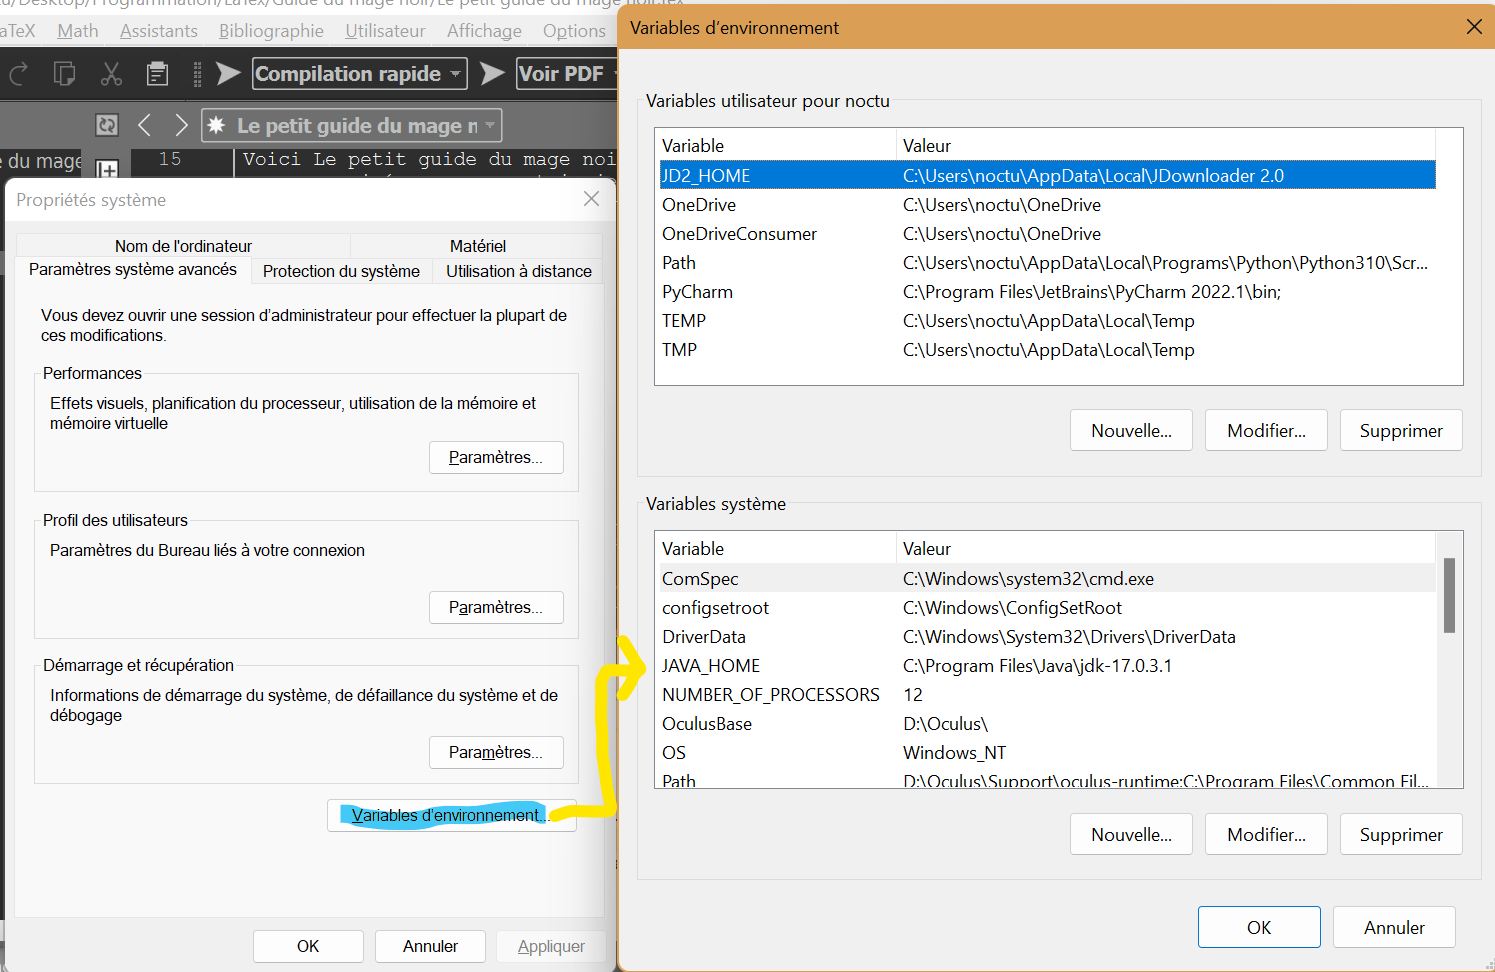
\includegraphics[scale=0.5]{img/env_var.png}
\end{figure}

Une fois que vous avez trouvé la bonne variable(si elle n'y est pas, vous pouvez la créer en cliquant sur "Nouvelle..."), changez sa valeur au dossier d'installation de votre java 17. Par défaut il est dans Programmes/Java, mais si vous avez changé son dossier d'installation, mettez ce chemin dans la variable. Il est possible qu'un redémarrage soit nécessaire pour que le changement soit effectif.

\subsection{MongoDB}
Maintenant que java est installé et configuré, on passe à MongoDB.\newline
MongoDB vous servira à gérer la base de données de votre serveur, vous pourrez vous servir de MongoDB Compass pour y accéder et la modifier.\newline
\href{https://fastdl.mongodb.org/windows/mongodb-windows-x86_64-5.0.7-signed.msi}{\textcolor{blue}{Le lien de MongoDB}}\newline
Lors de l'installation, il vous faudra vous assurer que MongoDB est bien installé en temps que service. Si vous ne le faites pas, il est possible que vous ayez des difficultés plus tard. Accessoirement, si l'on vous propose d'installer MongoDB Compass, dites oui, c'est toujours utile.

\subsection{Le proxy}
Pour le proxy, vous avez deux solutions:
\begin{itemize}
	\item Fiddler
	\item Mitmproxy
\end{itemize}
Personnellement je vous recommande mitmproxy car il se lancera automatiquement lors du lancement du serveur, alors que Fiddler devra être lancé à la main à chaque fois.

\subsubsection{Fiddler}
Si vous choisissez d'utiliser Fiddler, il vous faudra \href{https://www.telerik.com/download/fiddler/fiddler4}{\textcolor{blue}{télécharger Fiddler classic.}}\newline
Une fois l'installation faite, allez dans tools puis HTTPS et cochez "Capture HTTPS CONNECTs" ainsi que "Decrypt HTTPS traffic"\newline
Puis, toujours dans les options allez dans connections et changez "Fiddler Classic listens on port" à autre chose que 8888.\newline
Ensuite fermez les options et sur la page principale, là où il y a vraiment beaucoup d'onglets, cliquez sur FiddlerScript et remplacez tout le script déjà présent par \href{https://github.lunatic.moe/fiddlerscript}{\textcolor{blue}{celui-ci}} et cliquez sur "Save Script".\newline
Fiddler est maintenant configuré!

\subsubsection{Mitmproxy}
Pour Mitmproxy il n'y a rien à faire si vous pensez utiliser Grassclipper(ce que je recommande à 4000\% si vous voulez pas vous embêter)

\hrulefill

\section{Installation de Grasscutter}

\subsection{Version normale}
La version normale fait référence à la version stable, pas besoin de build le jar ici.

\subsubsection{Le jar de Grasscutter}
Pour commencer, il va vous falloir le .jar de Grasscutter, récupérez la dernière version \href{https://github.com/Grasscutters/Grasscutter/releases}{\textcolor{blue}{ici}}(prenez bien la dernière version stable, et pas une version dev).

\subsubsection{Les ressources}
Pour démarrer Grasscutter il vous faudra des ressources, que vous pouvez trouver \href{https://github.com/Koko-boya/Grasscutter_Resources/tree/main}{\textcolor{blue}{ici}}. Pour les récupérer via github: cliquez sur code puis "download ZIP".

\subsubsection{Les autres fichiers requis}
Une fois les ressources en votre possession, il va vous manquer d'autres petits fichiers, à savoir:
\begin{itemize}
	\item Les data
	\item Les keys
	\item Le keystore.p12
\end{itemize}

Pour les obtenir, je vous recommande de télécharger l'archive de la \href{https://github.com/Grasscutters/Grasscutter/tree/stable}{\textcolor{blue}{branche stable de Grasscutter}}(code puis "download ZIP").\newline
Une fois tout ceci en votre possession, vous pouvez passer à l'installation de Grasscutter!

\subsubsection{Installation de Grasscutter(stable)}
Maintenant que vous avez tous les pré-requis, il est temps de passer à l'installation.\newline
Commencez par mettre le .jar de Grasscutter dans un dossier vide, renommez le en grasscutter.jar pour simplifier.\newline
Ensuite créez un dossier resources, et placez-y les ressources que vous aviez téléchargées.\newline
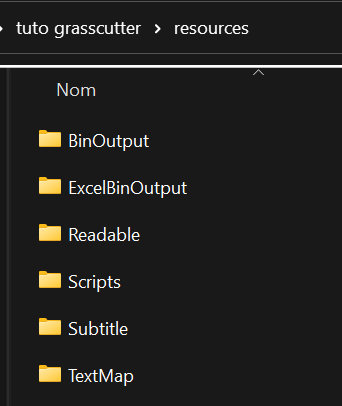
\includegraphics[scale=1]{img/disp_resources.png}\newline
Maintenant, les autres fichiers, déposez à la racine du dossier du serveur les dossiers "data", "keys" ainsi que le fichier "keystore.p12"\newline
Vous êtes bons pour pouvoir lancer le serveur maintenant

\subsection{Version beta(2.7)}
La version beta vous permettra d'accéder à la version 2.7 pour l'instant. C'est pas forcément plus compliqué à installer, juste un peu plus instable, et ça utilise des ressources différentes.

\subsubsection{Le jar de Grasscutter}
Voici le \href{https://drive.google.com/file/d/1cJJUqYeeMITWMGaZNTfPB751rEgFEui3/view?usp=sharing}{\textcolor{blue}{lien}}.\newline

\subsubsection{Les ressources}
Voici le \href{https://github.com/Koko-boya/Grasscutter_Resources/tree/2.7}{\textcolor{blue}{lien}}, cliquez sur code puis download ZIP pour les télécharger.\newline

\subsubsection{Les autres fichiers}
Vous pouvez télécharger ces fichiers \href{https://drive.google.com/file/d/12UwtBJnrxg1ZoNRVzXu9evL707Pi0bem/view?usp=sharing}{\textcolor{blue}{ici}}.

\subsubsection{Le client}
Cette méthode sera invalide dès la mise à jour officielle vers la 2.7.\newline\newline
Vous pouvez trouver le client 2.7 \href{https://www.reddit.com/r/Genshin_Impact/comments/uyou43/direct_download_links_for_genshin_impact_27_from/}{\textcolor{blue}{ici}}, il y a aussi les packs de langue si vous voulez.

\subsubsection{Installation de Grasscutter(beta)}
Commencez par placer le .jar de grasscuter dans un dossier vide, renommez-le en "grasscutter.jar".\newline
Ensuite créez un dossier resources et mettez-y les ressources de la 2.7.(voir image sur la version stable parce que c'est pareil et que j'ai la flemme d'en faire une exprès)\newline
Placez maintenant le dossier data et le fichier keystore.p12 à la racine de votre dossier Grasscutter.	\newline
Le lancement est classique, juste qu'il vous faudra lancer l'exécutable du client 2.7 à la place.

\hrulefill

\section{Lancement du serveur}
Il y a deux méthodes pour lancer le serveur:
\begin{itemize}
	\item Lancer via le cmd avec une commande
	\item Lancer via Grassclipper, qui est un launcher
\end{itemize}
Grassclipper est bien plus simple car il vous permettra d'ignorer le lancement du proxy car il se lancera tout seul(à choisir donc si vous n'utilisez pas Fiddler)

\subsection{Lancement via CMD}
Pour lancer via le CMD, il suffit d'ouvrir un terminal dans le dossier de Grasscutter(là où il y a le grasscutter.jar) et de lancer cette commande: "java -jar grasscutter.jar"(sans guillemets). Le serveur devrait se lancer, mais il vous faudra un proxy pour y accéder(Fiddler est préféré ici).

\subsection{Lancement via Grassclipper}
Grassclipper est un launcher tout en un, qui vous permettra à la fois de lancer votre serveur, mais aussi le jeu et le proxy en même temps!

\subsubsection{Téléchargement et configuration}
Commencez par prendre la dernière version de Grassclipper, disponible \href{https://github.com/Grasscutters/GrassClipper/releases}{\textcolor{blue}{ici}} et décompressez tout dans un dossier vide.\newline
Lancez maintenant GrassClipper.exe.\newline
Une fois lancé, vous devriez voir ceci:\newline
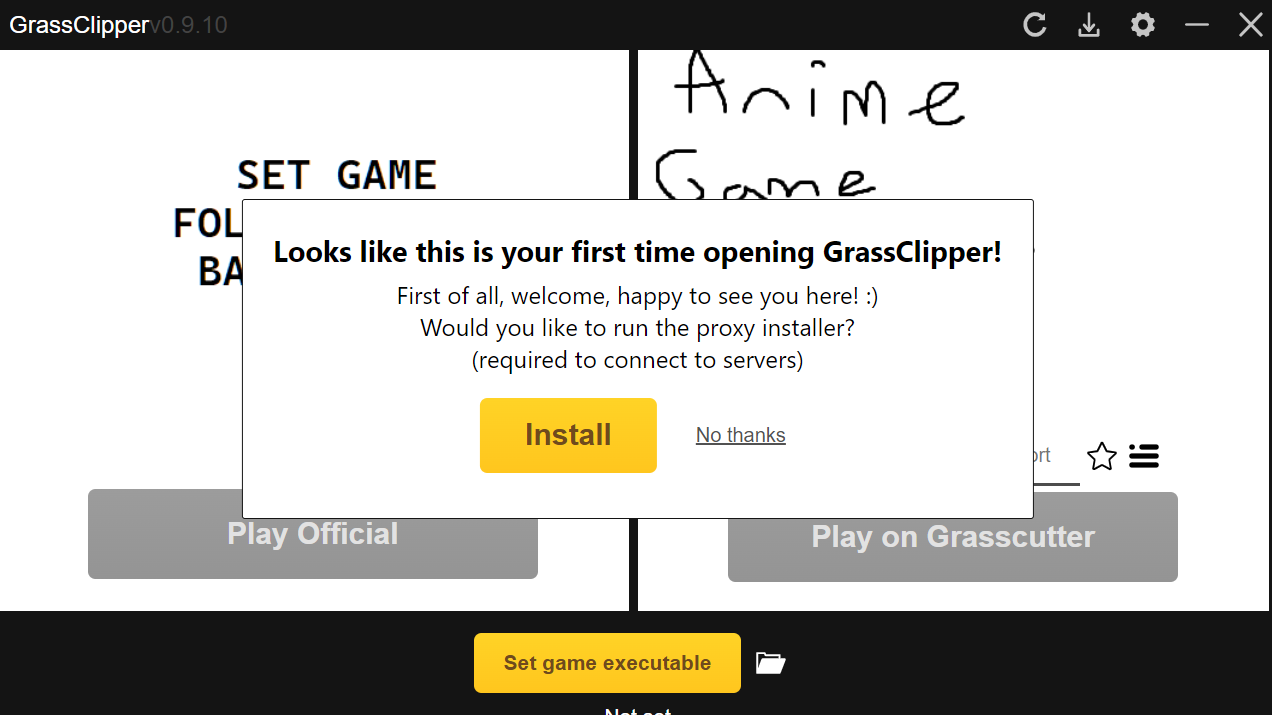
\includegraphics[scale=0.5]{img/first_grassclipper_use.png}\newline
Cliquez sur install, Grassclipper vous installera Mitmproxy.\newline
Si vous voyez cette erreur:\newline
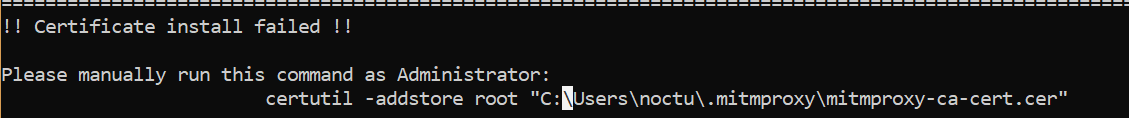
\includegraphics[scale=0.5]{img/error_cert.png}\newline
Lancez un terminal en mode administrateur et lancez la commande qu'il vous indique.
\newline\newline

Après avoir installé le proxy, vous allez devoir indiquer à Grassclipper où est votre jeu(je vous recommande très fortement de ne pas utiliser la même installation du jeu pour jouer sur les serveurs officiels ou sur votre serveur privé), vous devrez indiquer l'exécutable du jeu, et non du launcher du jeu.\newline
Une fois ceci fait, il vous faudra indiquer à Grassclipper que vous souhaitez lancer le serveur depuis Grassclipper. Il faut donc aller dans les options(le petit rouage en haut à droite), et cocher "enable server launcher". Vous pouvez aussi changer la langue de Grassclipper(le français est disponible).\newline
Vous devriez maintenant voir une nouvelle partie sur la fenêtre de Grassclipper, cliquez sur "set "Grasscutter" .jar file" et indiquez où se trouve le jar de Grasscutter. 

\subsubsection{Lancement}
Une fois Grassclipper et Grasscutter configurés, cliquez sur "Launch local server", votre serveur se lancera. Il devrait vous demander quelle langue vous voulez, marquez l'abréviation de votre choix. Si vous voyez "[INFO] Game Server started on port 22102", c'est que c'est bon, sinon reportez-vous à la section sur la résolution des problèmes.\newline
Cliquez maintenant sur "Play on Grasscutter", le proxy ainsi que le jeu se lanceront.

\hrulefill

\section{Après avoir lancé le jeu}
Voici quoi faire après avoir lancé le jeu!

\subsection{Création de compte}
Une fois le jeu lancé(et le serveur aussi bien entendu), il va vous falloir un compte, pour ça, rien de plus simple: rendez vous dans la console du serveur et rentrez ceci(modifiez avec vos propres valeurs)\newline
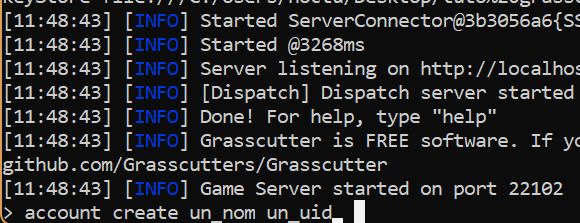
\includegraphics[scale=0.8]{img/account_create.png}\newline
À savoir que l'UID est facultatif, si vous ne le rentrez pas, il sera attribué automatiquement.\newline\newline

Après avoir créé votre compte, il ne reste plus qu'à vous connecter, rentrez votre nom d'utilisateur et en tant que mot de passe, n'importe quoi.\newline
Voilà, cliquez sur la porte, vous devriez voir la cinématique de début du jeu!

\hrulefill

\section{Extra}
Vous trouverez ici des petits extras, comme la génération du handbook par exemple!

\subsection{Le handbook}
Le handbook vous servira à retrouver tous les IDs, que ce soit les personnages, les matériaux ou les armes.\newline
Pour le générer, ouvrez un terminal dans le dossier de Grasscutter, et rentrez "java -jar grasscutter.jar -handbook". Un fichier du nom de "GM\_Handbook.txt" devrait être apparu dans le dossier de Grasscutter.\newline
Le handbook ne peut pas être généré avec la version 2.7(je n'ai pas réussi personnellement), il vous faudra le récupérer sur le \href{https://discord.gg/ZwKEJn7sxT}{\textcolor{blue}{discord}}.

\subsection{Les commandes}
Une liste des commandes est disponible \href{https://github.com/Grasscutters/Grasscutter/wiki/Commands}{\textcolor{blue}{ici}}

\subsection{Le multijoueur}
Alors ça, ça va attendre parce que j'ai tout essayé, ça veut pas marcher.

\hrulefill

\section{Les problèmes}
Cette section vous propose des solutions aux divers problèmes que vous pourrez rencontrer.

\subsection{Grasscutter}
Des problèmes avec le serveur? C'est ici!

\subsubsection{[WARN] Failed to load language file: fr-FR.json}
Si vous rencontrez cette erreur, c'est tout à fait normal, car il y a un bug sur la version stable 1.1.0, et il vous faudra altérer un peu la configuration du serveur.\newline
Ouvrez le config.json et allez à cette ligne là: "LocaleLanguage": "fr\_FR"," et changez le "fr\_FR" par "en\_US".\newline
Si vous ne la trouvez pas, elle est tout en bas normalement.

\subsection{Grassclipper}
Des problèmes avec Grassclipper? C'est ici!

\subsubsection{Une fenêtre totalement blanche}
Si vous voyez une fenêtre entièrement blanche lorsque vous lancez Grassclipper, il vous faut \href{https://developer.microsoft.com/en-us/microsoft-edge/webview2/#download}{\textcolor{blue}{ceci}}

\end{document}
